\section {Конструкторский раздел}
Для проверки работоспособности схемы необходимо собрать статистически значимое число образцов. 
VirusShare \cite{VIRUSSHARE} предоставляет доступ к коллекции вредоносных образцов за 2011-2015, полученных от различных производителей антивирусов, HoneyPot'ов и других источников, собранных в пачки по 65536 штук.
MalShare Project \cite{MALSHARE} предоставляет доступ на скачивание  всего до 1000 образцов из их хранилища в день, однако у них новые образцы появляются практически ежедневно.

В связи с этим, было принято решение о первоначальном сборе логов на пачках из VirusShare (''обучающая`` выборка) и последующей проверке обнаружения цепочек на собираемых ежедневно с начала 2016 года образцов из MalShare (''тестовая`` выборка). В связи с имеющимися в наличии ресурсами представляется возможным прогнать всего порядка 60000 штук, поэтому разделим выборки на 56634 vs 7657 штук.

После сбора логов и преобразования становится возможным проследить некоторые тенденции в собранных данных. Если посмотреть на график \ref{fig:seq_len_hist}, видно, что значительную часть собранных цепочек составляют те, у которых число вызовов 132 и менее. Скорее всего, большая часть из них относится к тем образцам, у которых по тем или иным причинам не удалось собрать достаточно полную картину вызовов, будь то из-за внезапного завершения работы, проблем обнаружения точки входа упакованных образцов, или каким-либо иным. Длина цепочек большей длины приблизительно соответствует по форме нормальному распределению, а при увеличении числа образцов следовало бы ожидать большей схожести.

\begin {figure}[ht]
        \centering
        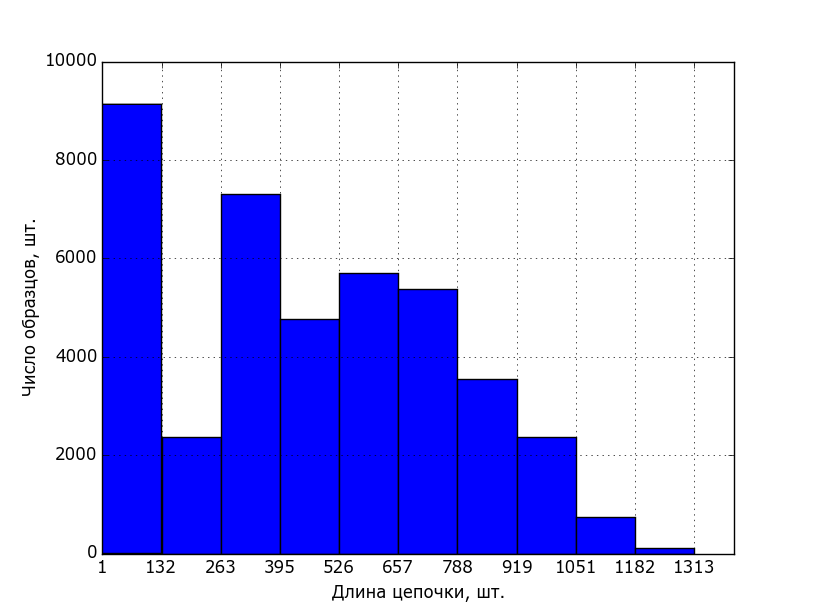
\includegraphics[width=\linewidth] {img/sequence_len_hist.png}
        \caption {Распределение длины цепочек среди образцов}
        \label {fig:seq_len_hist}
\end {figure}




